
\FloatBarrier
\section{Система Чуа} % _CHUA_

\LinkRef{
 chua: ASAU-18, MKMM-2014, APIR-2011
}

Одной из известных хаотических систем, легко реализуемых как модельно (\ref{atu:eq:chua}),
так и схемотехнически (рис.~\ref{atu:f:chuascheme}),
является нелинейная система Чуа~\cite{moon_chaotic_vibr,buga_chua,Kennedy92robustop}:

\begin{figure}[htb!]
\begin{center}
% vi:syntax=tex

\begin{circuitikz}[line width=0.7]
  \ctikzset{bipoles/thickness=2}
  \def\Top{3.0}
  \draw (0.0,0.0) to[L,l=$L$,i=$I_L$] (0,\Top)
   to[R=R] (6.0,\Top)
   to[ageneric,l=$R_c$] (6.0,0.0) -- (0.0,0.0);
  \draw(1.5,0.0) to[C,l=$C_2$,v=$V_2$] (1.5,\Top );
  \draw(4.5,0.0) to[C,l=$C_1$,v=$V_1$] (4.5,\Top );
\end{circuitikz}

% \begin{tikzpicture}[circuit ee IEC,very thick,circuit symbol unit=3.5mm]
%   \node (L1) at (0,1.5) [point up,elelem,inductor={info = $L$}] {};
%   \node      at (0.2,2.4) {$I_L$};
%   \node (C2) at (1.5,1.5) [point up,elelem,capacitor={info = $C_2$}] {};
%   \node      at (1.8,1.8) {$V_2$};
%   \node (pc2d) at (1.5,0) [contact] {};
%   \node (pc2u) at (1.5,3) [contact] {};
%   \node (C1) at (5.0,1.5) [point up,elelem,capacitor={info = $C_1$}] {};
%   \node      at (5.3,1.8) {$V_1$};
%   \node (pc1d) at (5,0) [contact] {};
%   \node (pc1u) at (5,3) [contact] {};
%   \node (R) at (3,3) [elelem,resistor={info = $R$}] {};
%   \node (Rc) at (7,1.5) [elelem,point up,resistor={info = $R_c$}] {};
%   \draw (Rc) ++(-0.15,-0.7) rectangle+(0.3,0.2);
%   \draw (L1) |- (pc2d) -- (pc1d) -| (Rc) [wire];
%   \draw (L1) |- (pc2u) -- (R) -- (pc1u) -| (Rc) [wire];
%   \draw (pc2u) -- (C2) [wire]; \draw (pc2d) -- (C2) [wire];
%   \draw (pc1u) -- (C1) [wire]; \draw (pc1d) -- (C1) [wire];
%   \node (Gr) at (5,-0.3) [elelem,point down,ground] {};
%   \draw (pc1d) -- (Gr) [wire];
% \end{tikzpicture}

\end{center}
\caption{Условная электрическая цепь, реализующая хаотическую систему Чуа}
\label{atu:f:chuascheme}
\end{figure}


\begin{equation}
\begin{cases}
  C_1 \dot{V_1}  = \frac{1}{R} ( V_2 - V_1 ) - g(V_1), \\
  C_2 \dot{V_2}  = \frac{1}{R} ( V_1 - V_2 ) + I_L, \\
  \dot{I_L}      = - \frac{1}{L} V_2 .
\end{cases}
\label{atu:eq:chua}
\end{equation}

Единственным нелинейным элементом в данной системе является ``диод Чуа''
(обозначен на схеме как $R_c$) с
характеристикой $g(V)$~(рис.~\ref{atu:f:diodchua}),
обладающей различным отрицательными наклонами
($m_0$ и $m_1$) на разных участках,
и тем самым являющийся управляемым источником энергии.
%
%
\begin{equation}
g(V) =
\begin{cases}
  m_1 V = ( m_0 + m_2 ) V , & |V| <   U_0, \\
  m_0 V ,                   & |V| \ge U_0.
\end{cases}
\label{atu:eq:diodchua}
\end{equation}

\begin{figure}[htb!]
\begin{center}
% vi:syntax=tex
\begin{tikzpicture}
  \coordinate (XMIN) at (-4.5,0.0);
  \coordinate (XMAX) at ( 4.5,0.0);
  \coordinate (YMIN) at (0,-2.5);
  \coordinate (YMAX) at (0, 2.5);
  \draw (XMIN) -- (XMAX) [medline,->] node[below] {$U$};
  \draw (YMIN) -- (YMAX) [medline,->] node[left]  {$I$};
  \draw (-4,2) -- (-1,1) -- (1,-1) -- (4,-2) [boldline];
  \draw (1,-1) -- (1,0) [dashed,medline];
  \draw (1,-1) -- (4,-1) [dashed,medline];
  \draw (1.41,0) arc [medline,->,start angle=0,end angle=-45,radius=1.41];
  \draw (1,-1) ++(2,0) arc [medline,->,start angle=0,end angle=-18,radius=2.0];
  \filldraw (1,0) circle[radius=0.05,fill=black] node[above] {$U_0$};
  \node[right] at (1.2,-0.6) {$\alpha_1: \tan(\alpha_1)=m_1$};
  \node[right] at (3.0,-1.3) {$\alpha_0$};
\end{tikzpicture}

\end{center}
\caption{Характеристика \(I=g(V)\) диода Чуа}
\label{atu:f:diodchua}
\end{figure}


При этом параметр \(m_0\) определяет поступление энергии в систему
при больших амплитудах \(V_1\), и, в целом, характеризует
энергетические возможности источника.
Аналогично, параметр \(m_1\) характеризует поступление энергии
при малых колебаниях, в частности, определяет, будет ли
система переходить в колебательное состояние при малых начальных
возмущениях, и какой будет режим этих колебаний.
С другой стороны, поскольку параметр \(m_1\) является суммой
``глобального параметра'' \(m_0\) и ``довеска'',
определяющего дополнительный вклад при малых амплитудах,
то имеет смысл перейти от параметра \(m_1\) к параметру
\( m_2 = m_1 - m_0 \), который
и определяет в целом нелинейность
системы. При \( m_2 = 0 \) система становится линейной
и не представляет особого интереса. Поэтому
в данной работе в качестве
идентифицируемого параметра рассматривается именно параметр \(m_2\).

Важно, что в зависимости от величины параметра $m_2$,
система может переходить в режимы затухания,
периодического и сложно-периодического движения, а также в режим
хаотических колебаний~\cite{anisch_nonlin_eff,magni_new_meth}. При этом сложно-периодическое и хаотическое
движения чередуются с изменением величины \(m_2\).


Классически параметры системы Чуа задаются следующим образом~\cite{buga_chua}:
$C_1 = 1/9$, $C_2 = 1$, $L= 1/7$, $R = 1/0.7$, $m_0=-0.5$, $ m_2 \in [ -0.15; -0.7 ] $.

Введём обозначения:
\[
  a_{11} = \frac{1}{R C_1}; \;
  a_{13} = \frac{1}{C_1}; \;
  a_{21} = \frac{1}{R C_2}; \;
  a_{23} = \frac{1}{C_2}; \;
  a_{31} = -\frac{1}{L}; \;
  a_g = - \frac{m_0}{C_1}; \;
  \mu = - \frac{m_2}{C_1}.
\]
%
%\noindent
Тогда:
%
\begin{equation}
\begin{cases}
  \dot{V}_1  = -a_{11} V_1 + a_{11}  V_2  + g_1(V_1) , \\
  \dot{V}_2  = +a_{21} V_1 - a_{21}  V_2  + a_{23} I_L    , \\
  \dot{I}_L  =  a_{31} V_2.
\end{cases}
\label{atu:eq:chua2}
\end{equation}
%
%
\begin{equation}
g_1(V) =
\begin{cases}
  ( a_g + \mu ) V , & |V| <   U_0, \\
  a_g V           , & |V| \ge U_0.
\end{cases}
\label{atu:eq:diodchua2}
\end{equation}

При этом пересчитанные классические значения параметров будут представлены следующим образом:
$ a_{11} = 6.5 $, $a_{21} = 0.7$, $ a_{23} = -7 $, $ a_g = 4.5 $,
$ \mu \in [ 1.29 ; 5.6 ] $.
Соответственно, в этих обозначениях
идентифицируемым параметров является $\mu$.



\begin{figure}[htb!]
\centerline{
  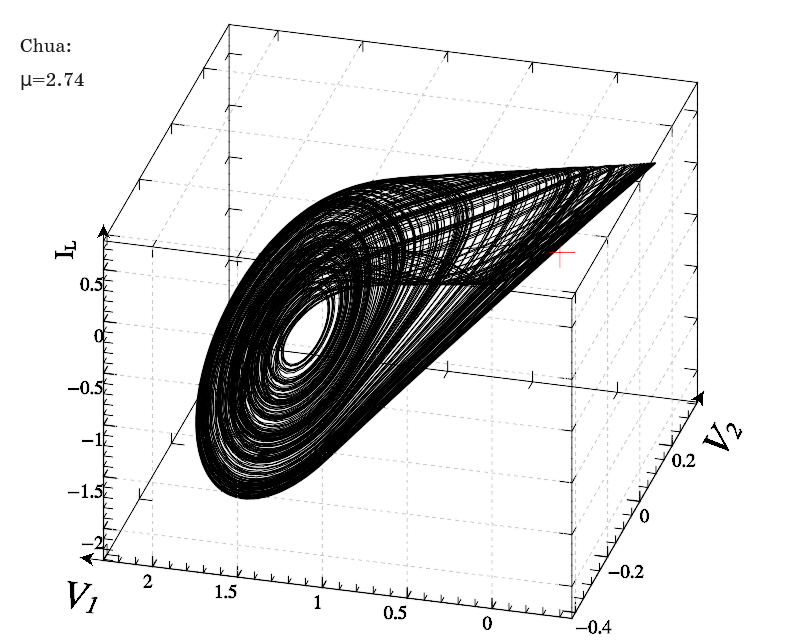
\includegraphics[width=0.49\textwidth]{p/cha/chua/chua_1-p_xyz_mu=2x74.png}
  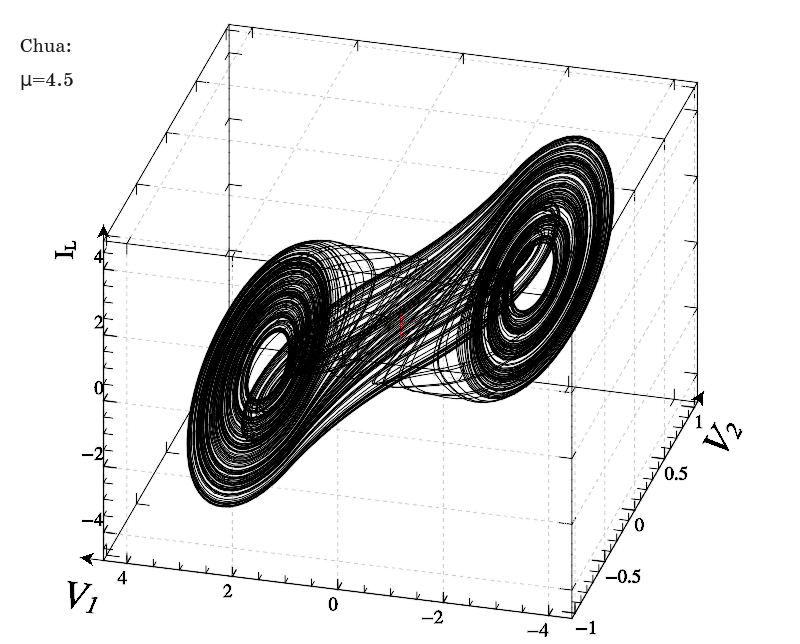
\includegraphics[width=0.49\textwidth]{p/cha/chua/chua_1-p_xyz_mu=4x50.png}
}
\caption{Аттрактор системы Чуа (\ref{atu:eq:chua2}) при различных значениях $\mu$}
\label{atu:f:chua_phase}
\end{figure}


Для определения вида критерия рассмотрим зависимости
$q_{*}(\mu) $ (индексом ``*'' будем обозначать применение какого-либо из индексов,
обозначающих исходный сигнал для критерия и способ усреднения),
полученные путём моделирования
для системы Чуа (рис.~\ref{atu:f:chua_q}):

\begin{figure}[htb!]
\centerline{
  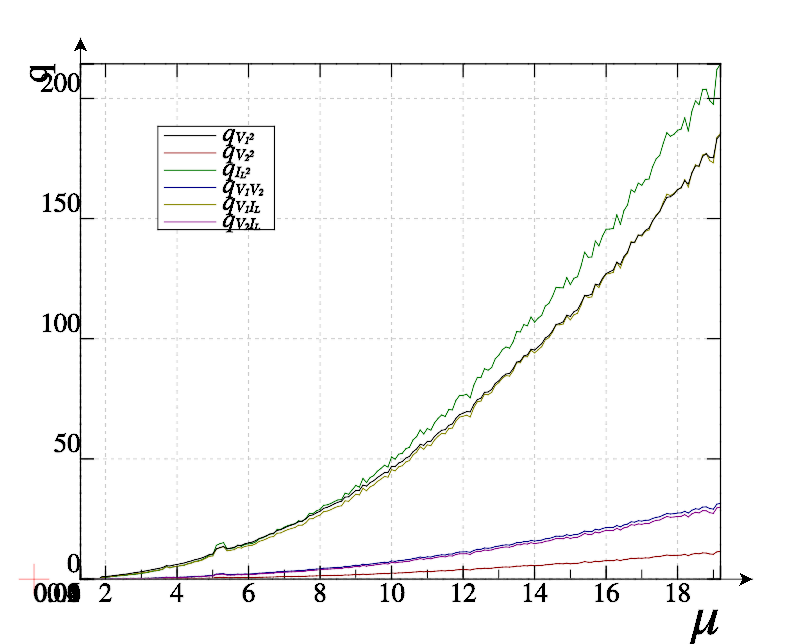
\includegraphics[width=0.49\textwidth]{p/cha/chua/chua_q-p_mu2.png}
  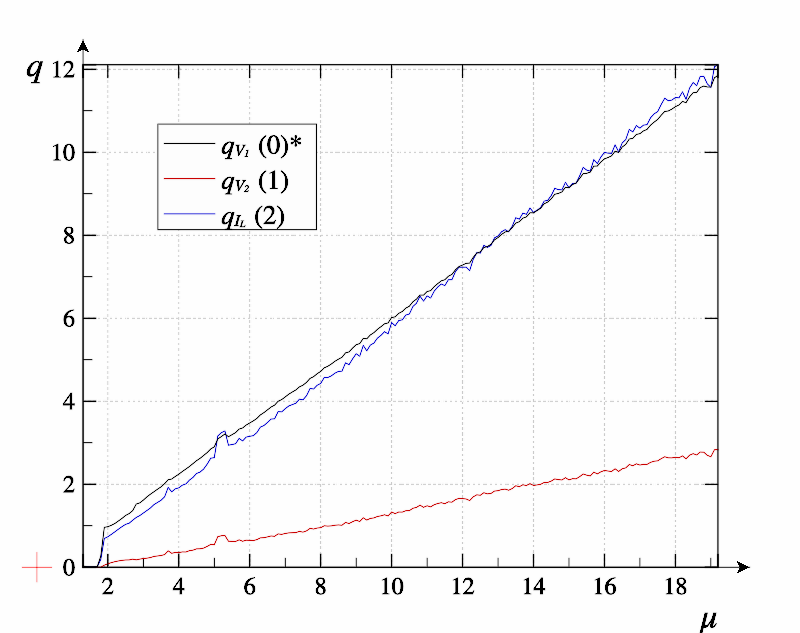
\includegraphics[width=0.49\textwidth]{p/cha/chua/chua_q-p_mu1.png}
}
  \caption{Зависимости $q_{*}(\mu) $ для системы Чуа (\ref{atu:eq:chua2})}
\label{atu:f:chua_q}
\end{figure}

Из графиков очевидно, что величина $ q_{V_1}(\mu) $
является наилучшим кандидатом в критерии, ввиду близкой к линейной зависимости
в рабочем диапазоне.

Следующим важным параметром, необходимым для эффективной работы системы идентификации, является
характерное время время оценивания $\tau$ (\ref{atu:eq:qlin}), или же обратная ему величина $a_q$.

Для предварительного оценивания величины $a_q$ рассмотрим спектры системы при различных
$\mu$ (рис.~\ref{atu:f:chua_spectrum}). Как следует из графиков, спектр системы достаточно
ограничен сверху, однако, в хаотическом режиме является сплошным практически до нуля.
Это не даёт возможности непосредственно определить $a_q$ исходя из спектра,
однако, первые существенные пики наблюдаются при $ \omega \approx 0.3 $, следовательно,
первоначальное значение $a_q$ можно оценить как $ a_q \approx 0.3 / \pi \approx 0.1 $.


\begin{figure}[htb!]
\centerline{
  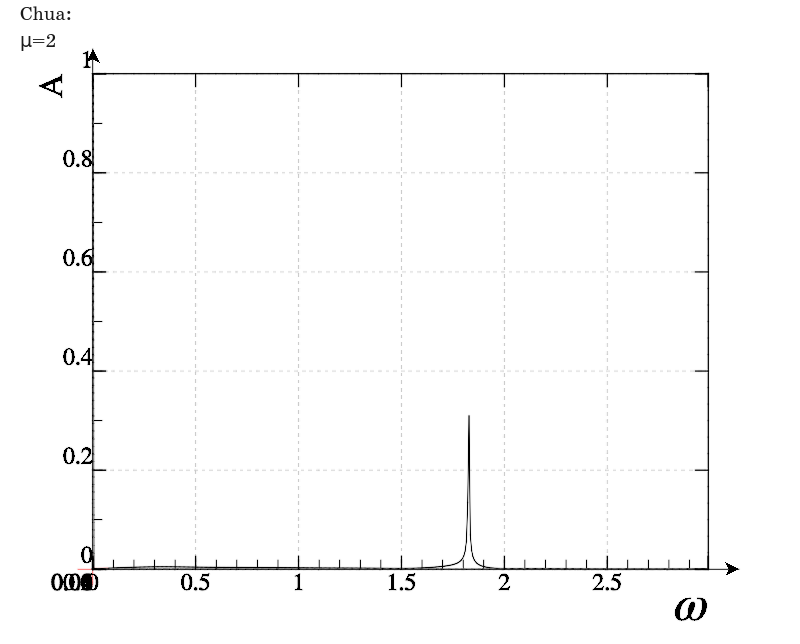
\includegraphics[width=0.32\textwidth]{p/cha/chua/chua_f-p_f_mu=2x00.png}
  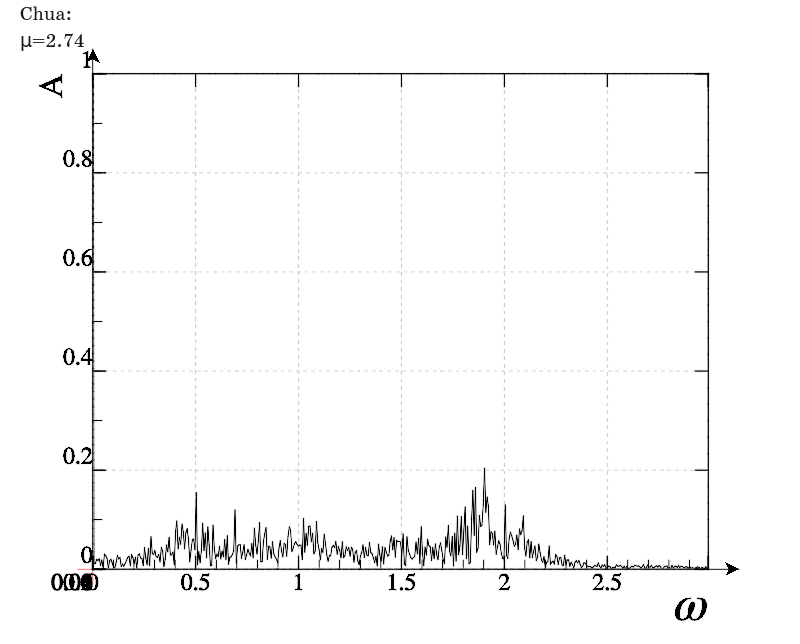
\includegraphics[width=0.32\textwidth]{p/cha/chua/chua_f-p_f_mu=2x74.png}
  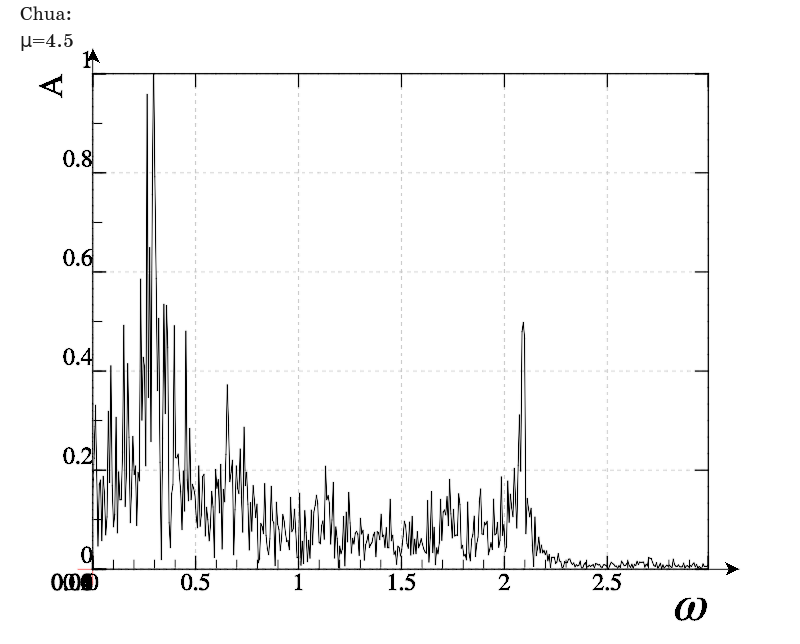
\includegraphics[width=0.32\textwidth]{p/cha/chua/chua_f-p_f_mu=4x50.png}
}
\caption{Спектры системы Чуа (\ref{atu:eq:chua2}) при различных значениях $\mu$}
\label{atu:f:chua_spectrum}
\end{figure}

Следующий способ оценить $a_q$ -- исследовать полученную в результате моделирования
зависимость среднеквадратичного отклонения $e_q$ оценки величины $q$, нормированной
на саму величину $q$ в стационарном случае. Полученная зависимость представлена
на рис.~\ref{atu:f:chua_tau}.

\begin{figure}[htb!]
\centerline{
  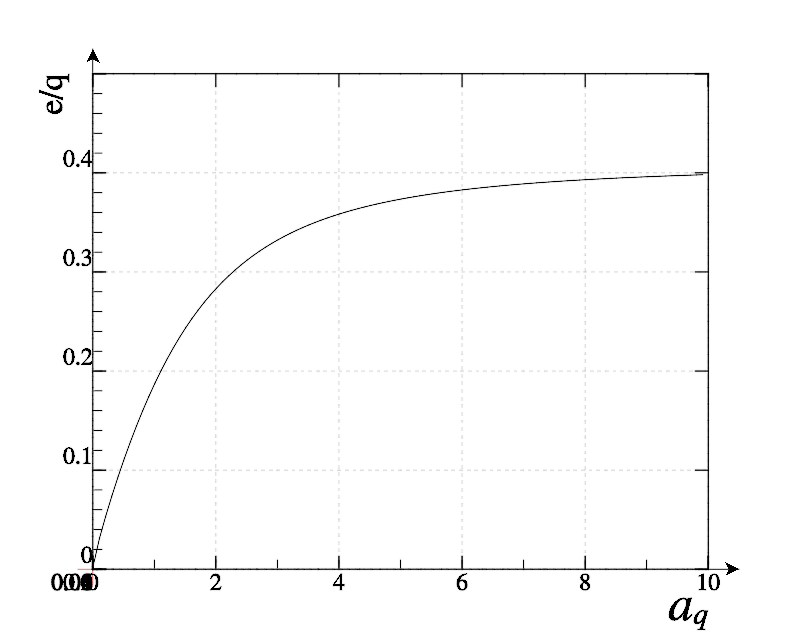
\includegraphics[width=0.4\textwidth]{p/cha/chua/chua_tau-p_e_a.png}
}
\caption{Типичная зависимость $e_q/q(a_q)$ для системы (\ref{atu:eq:chua2})}
\label{atu:f:chua_tau}
\end{figure}

Из этого графика можно сделать вывод, что первоначальная оценка $a_q$
была сделана корректно.

В качестве системы идентификации использовалась система с 5 поисковыми агентами и
двумя неподвижными моделями. Для исследования динамических свойств системы идентификации
параметр $\mu_o$ для объекта задавался двумя способами:
%
\begin{equation}
 \mu_o(t) = p_0 + U_p \sign \sin( \omega_p t )
  \label{atu:eq:chua_mu_sign}
\end{equation}
%
\begin{equation}
 \mu_o(t) = p_0 + U_p \sin( \omega_p t ).
  \label{atu:eq:chua_mu_sin}
\end{equation}

Динамика процессов идентификации для системы Чуа представлена на рис.~\ref{atu:f:chua_id}.


\begin{figure}[htb!]
\centerline{
  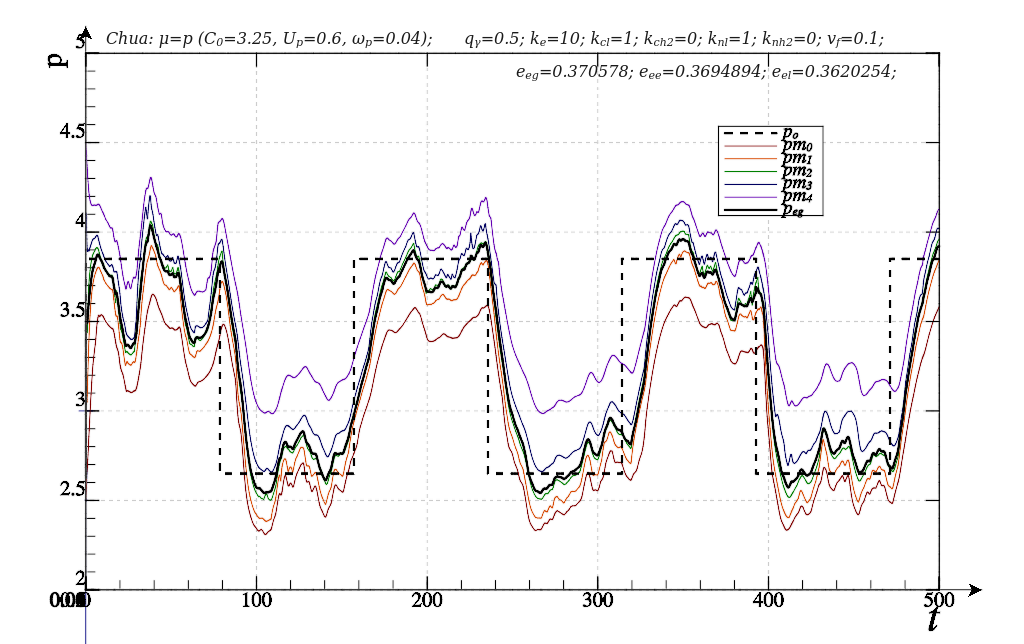
\includegraphics[width=0.49\textwidth]{p/cha/chua/chua_m5p-pl_n_sign.png}
  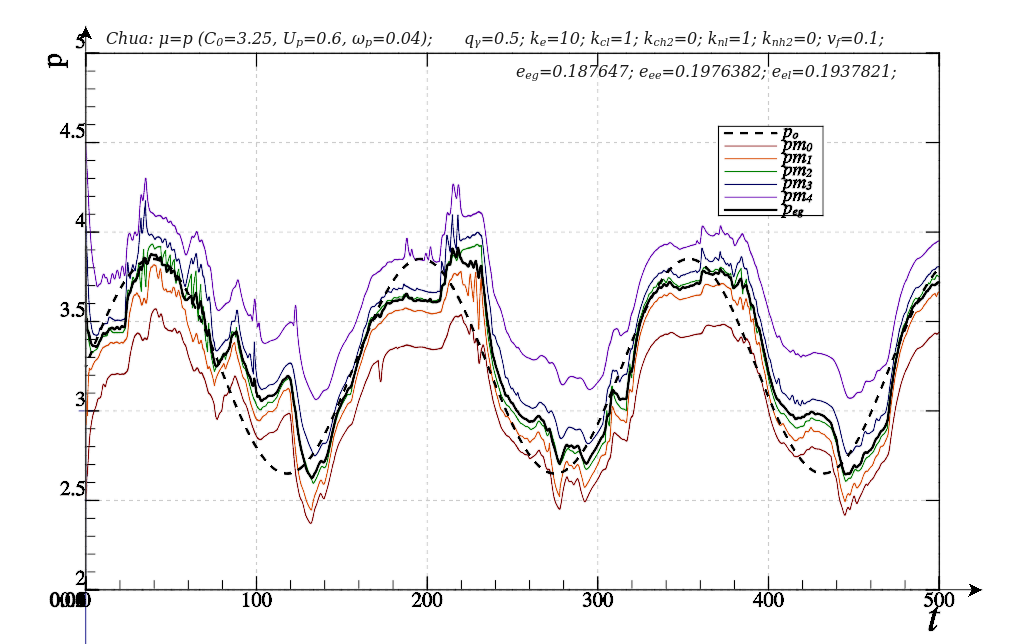
\includegraphics[width=0.49\textwidth]{p/cha/chua/chua_m5p-pl_n_sin.png}
}
\caption{Процесс идентификации параметра $\mu$ системы (\ref{atu:eq:chua2})
  при условиях (\ref{atu:eq:chua_mu_sign}) и (\ref{atu:eq:chua_mu_sin})
}
\label{atu:f:chua_id}
\end{figure}

Для более точной настройки параметров самой системы идентификации
рассмотрим зависимости среднеквадратических ошибок идентификации
от основных параметров системы идентификации.

Одним из важнейших параметров является $q_\gamma$ -- масштаб функции качества
((\ref{atu:eq:F_gauss})--(\ref{atu:eq:F_log})).
Зависимости для этого параметра приведены на рис.~\ref{atu:f:chua_e_qgamma}.

\begin{figure}[htb!]
\centerline{
  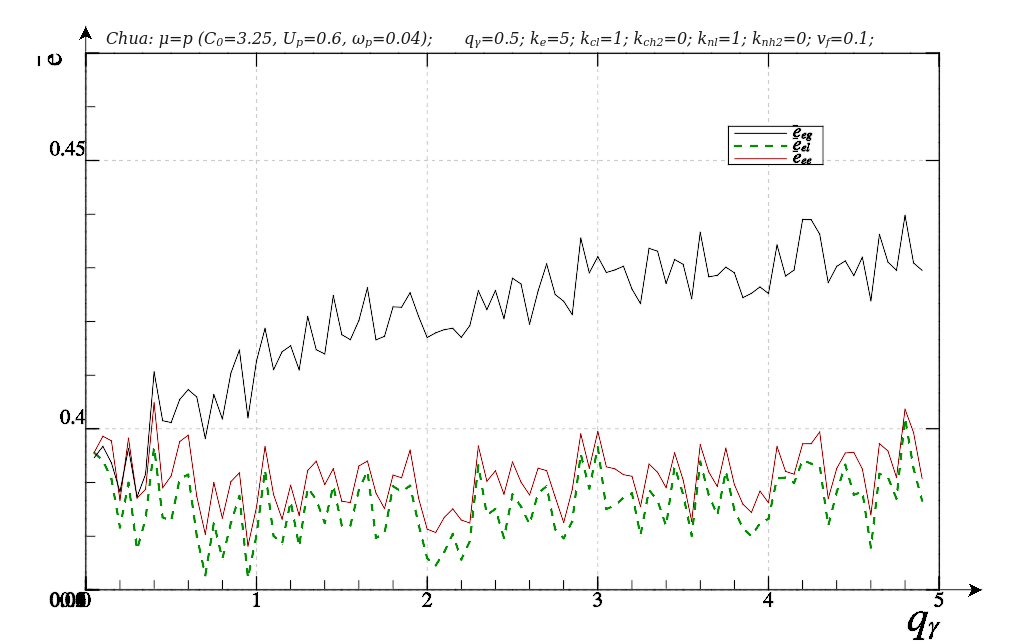
\includegraphics[width=0.49\textwidth]{p/cha/chua/chua_m5p-p_qg_e_sign.png}
  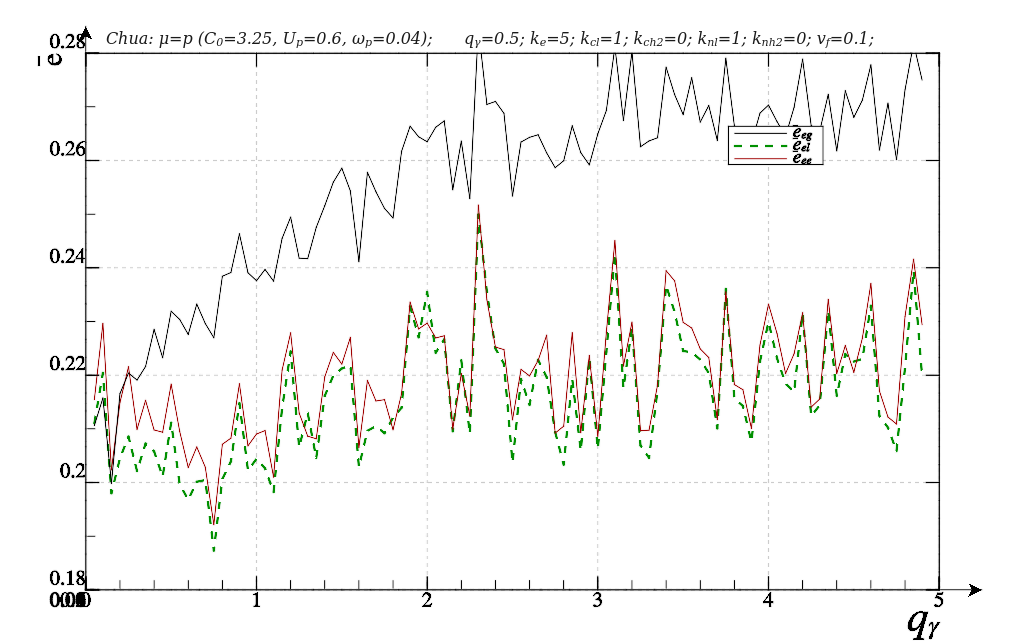
\includegraphics[width=0.49\textwidth]{p/cha/chua/chua_m5p-p_qg_e_sin.png}
}
  \caption{Зависимости  $\overline{e}(q_\gamma)$ для системы (\ref{atu:eq:chua2})
  при условиях (\ref{atu:eq:chua_mu_sign}) и (\ref{atu:eq:chua_mu_sin})
}
\label{atu:f:chua_e_qgamma}
\end{figure}

Явно выраженного экстремума не наблюдается, что свидетельствует
о сильной робастности метода.

Для проверки корректности выбора величины $a_q$ была построены зависимости
среднеквадратических ошибок идентификации (рис.\ref{atu:f:chua_e_a_q}).


\begin{figure}[htb!]
\centerline{
  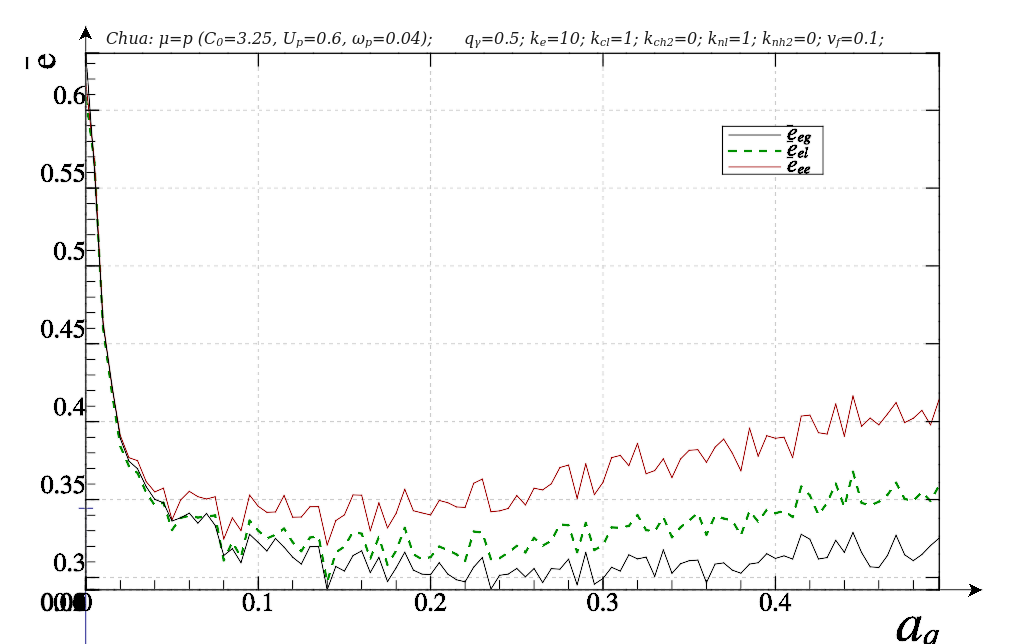
\includegraphics[width=0.49\textwidth]{p/cha/chua/chua_m5p-p_a_q_e_sign.png}
  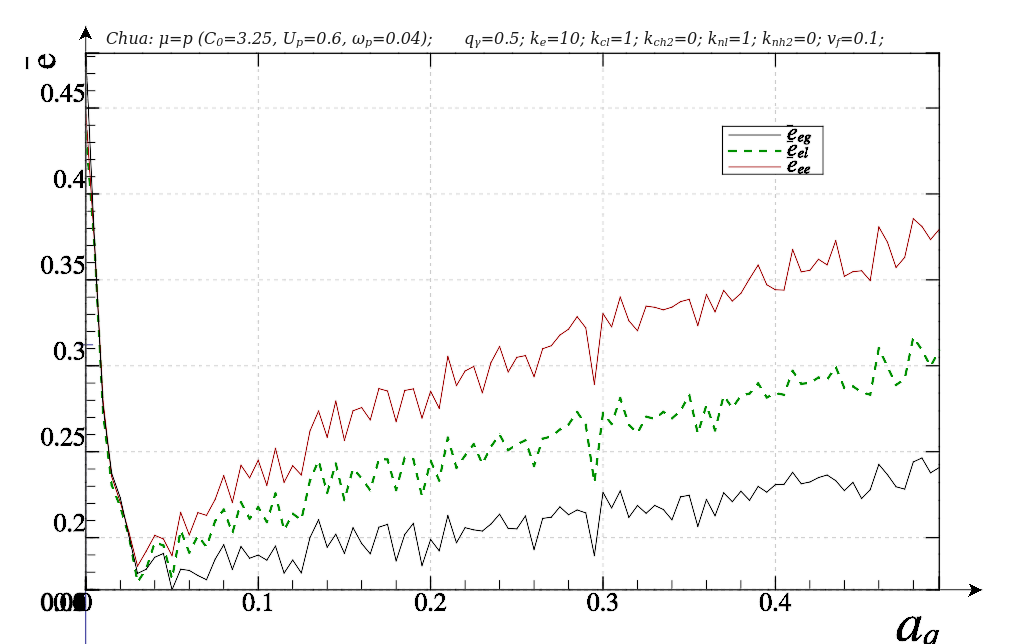
\includegraphics[width=0.49\textwidth]{p/cha/chua/chua_m5p-p_a_q_e_sin.png}
}
  \caption{Зависимости  $\overline{e}(a_q)$ для системы (\ref{atu:eq:chua2})
  при условиях (\ref{atu:eq:chua_mu_sign}) и (\ref{atu:eq:chua_mu_sin})
}
\label{atu:f:chua_e_a_q}
\end{figure}

Как видно, первоначальная оценка ``правильного'' значения величины $a_q$
была сделана достаточно точно. При этом, при синусоидальном изменении параметра объекта
меньшая ошибка идентификации наблюдается при меньших значениях $a_q$, что связано
с тем, в данном случае нет необходимости в слежении за скачкообразно изменяющимся параметром,
и, следовательно, допустимо большее время оценивания. Напротив, в случае (\ref{atu:eq:chua_mu_sign})
увеличение времени оценивания приводит к заметному снижению интегральной точности идентификации.


